\section{Algorithm construction}
\label{cha:Algorithm_construction}
In this section basic information about algorithm construction will be
presented. For the classification task three algorithms were implemented and
compared. At the beginning, we start with the basic algorithm of rough sets, later present rough sets
algorithm with modification of decision rules and at last the multistage hybrid 
algorithm consisting of genetic algorithm, rough sets and fuzzy logic is shown in 
greater details. 
\subsection{Rough sets algorithm construction}
\label{cha:Algorithm_construction_rough_set}
The basic rough sets algorithm with constant step of granulation
can be summarized in six steps \cite{bib34}, \cite{bib35}:
\begin{enumerate}
    \item Algorithm starts with an arbitrary chosen step of granulation which
        requires dividing every domain of feature into $G$ intervals.
        If the attributes are the real numbers then the granulation preprocessing 
        is needed first. To calculate the proper interval eq. (\ref{eq:interval})
        is used:
        \begin{equation}
            v_{pi}^{i} = \lfloor \frac{f_{i}}{G}\cdot(f_{i,
            max}-f_{i,min})\rfloor
            \label{eq:interval}
        \end{equation}
        where $v_{pi}^{i}$ is the interval label for $i$-th attribute; $f_i$ is
        the $i$-th real attribute value for pattern $x$, $f_{i,min}$ and
        $f_{i,max}$ denote the extend of the $i$-th feature calculated in the
        training phase and $\lfloor . \rfloor$ is the operator extracting
        integer value from real number. If for any attribute from $x$ in the testing phase 
        $f_i > f_{i, max}$ then $v_{pi}^{i}=G-1$ or $f_i < f_{i, min}$ then
        $v_{pi}^{i}=0$, in other cases eq. (\ref{eq:interval}) is applied.
        If the attributes are discrete then no preprocessing is required and 
        interval label is the same as feature discrete value.

        After this step, the value of each attribute is represented 
        by the number of interval in which this attribute is included. For each
        attribute from $l=(1, \ldots , q)$ we choose the same numbers of
        intervals $K_l$ called step of granulation $G$. For the $l$-th attribute 
        denoted by $v^l_{p_l}$ it is defined its $p_l$ interval from $p_l=(1, \ldots, K_l)$
    \item Using training dataset, construct the decision table $T$ where each
        row represents a pattern with additional class label. 
        Over the table $T$ define the set $FOR(C)$ of decision rules of
        the following form:
        $$IF \, (x_1 = v_{p_1}^1) \, AND \, (x_2=v_{p_2}^2) \, AND \, \ldots \,
        (x_q=v_{p_q}^q) \, THEN \, \Psi(S, x)=j$$
        Each generated rule is evaluated and the strength factor is assigned to
        it determining the accuracy of approximation (see section \ref{cha:Rough_sets_indicators})
    \item For the created set of formulas $FOR(C)$ for each $j=1, \ldots, m$
        an algorithm calculates lower $\underline{I_P}$, upper $\overline{I_P}$ approximations and the boundary
        region $BN_P$ which are determined by the set of conditional attributes $P
        \subseteq Q$ 
    \item In order to classify new pattern $x$ algorithm looks for matching rules in the
        set $FOR(C)$ (rule is activated if the left condition is fulfilled by
        attributes describing $x$).
    \item If there is only one matching rule $r$, then the pattern $x$ is
        classified to the class which is indicated by $r$-th decision attribute $j$, 
        because for sure such a rule is belonging to the lower approximation of all rules 
        indicating $j$. Rule $r$ is denoted as a \textit{certain} rule.
    \item If there is more than one matching rule in the set $For(C)$, 
        it means that the recognized pattern should be classified by the 
        rules from the boundary regions and in this case as a decision
        algorithm takes the index of boundary region for which the strength of corresponding 
        rule is maximal. All activated rules are denoted as \textit{possible}
        rules.
    \item In other cases: no appropriate rule was found or few rules have the same strength
        factor then the unknown pattern $x$ is rejected.
\end{enumerate}
\subsection{Rough sets algorithm construction with modification of decision rules}
\label{cha:Algorithm_construction_rough_set_modification}
It can happen that for particular number of intervals basic rough sets algorithm can not find patterns in
the training set, so as the consequence \textit{dummy} rules are generated, useless in the
classification process (the strength of the rule is 0). 
The main drawback of algorithm presented in section \ref{cha:Algorithm_construction_rough_set}
is the fact that it starts with an arbitrary chosen step of granulation and its accuracy strongly
depends on it. In this section the recursive modification of the previous algorithm is
presented for automatically changing the step of granulation if
the pattern $x$ is rejected. The modification is as follows \cite{bib36}:
\begin{enumerate}
    \item Algorithm starts with an arbitrary chosen step of granulation  $G$, 
        generally it is a high value to ensure that recursion can be invoked
        by decreasing $G$. At first algorithm repeats the whole procedure 1-6 described
        in the previous section.
    \item If for the pattern $x$ algorithm cannot find neither \textit{certain} nor \textit{possible}
        decision rule, it means that there is no proper representation in the learning set. 
        In such a situation algorithm tries to find matching rule by decreasing recursively
        the current interval $G$ by factor $\epsilon=1$ for every condition attribute $l=1, \ldots, q$
        until the proper rule is found. If \textit{certain} rule or
        \textit{possible} rules with maximum strength are induced then the algorithm
        returns decision attribute $j$, otherwise if for every attribute $G=1$, then the pattern $x$ is rejected.
\end{enumerate} 
The recursion is time consuming so to enhance the process of finding the proper
decision formulas for different $G$ the decision set $FOR(C)$ is stored in the memory
for faster retrieval.

\subsection{Multistage hybrid algorithm construction}
\label{cha:Multistage}
\subsubsection{Motivations}
\label{cha:Mutlistage_motivations}
When we deal with complex data it can happen that a single classifier is not
sufficient. There arises a question if connection of different classifier will
improve the classification? In this thesis the hybridization of rough sets and
fuzzy logic is proposed and investigated. The next subsections show algorithm construction.

\subsubsection{Fuzzy logic algorithm construction}
\label{cha:Algorithm_construction_fuzzy_logic}
\paragraph{Problem formulation}
\label{cha:Fuzzy_logic_basic_problem_formulation}
In the fuzzy logic algorithm one of the most important key is creation of rules
which will ensure correct classification. When there is no expert knowledge about
dataset it is not an easy task to generate them from scratch. In the literature
one can find many practical examples of how to generate \textit{IF-THEN} rules, from
the statistical tools to heuristic algorithms. In the recent years the most appealing
and effective approach is genetic algorithm \cite{bib4}, \cite{bib13}, \cite{bib23}.
For the algorithm construction we have to make few assumptions:
\begin{itemize}
    \item for the learning procedure $N$ training patterns are available,
    \item a set $F$ of linguistic values and their membership functions are given
        for describing each attribute.
\end{itemize}

From points enumerated above, the second one is the most important and the choice of the proper membership
functions affects the classification accuracy \cite{bib17}, \cite{bib6}. It requires in-depth explanation
of how set $F$ is generated in this thesis, how to partition each attribute into 
linguistic values and how to describe each membership function. Genetic
algorithm is used here for finding an optimal parameter settings. 

Fig. \ref{fig:fuzzy_example} shows an example of how to generate fuzzy set $F$ of
possible membership functions. In this example $14$ membership functions are used. 
Each function has a subscript defining its linguistic value and a proper
location in the feature space. To emphasize the complexity of the problem let take 
into account that each attribute is divided in the same way as depicted in fig. \ref{fig:fuzzy_example}. 
Having $d$-dimensional feature space, we would like to generate decision rules consisting of $d$ antecedents.
For each position we can choose 1 out of 14 membership functions which gives $14^d$ possibilities. 
It is impossible to evaluate each potential solution in a reasonable time, especially for greater $d$ \cite{bib27}, \cite{bib33}. 
\begin{figure}[H]
    \begin{center}
        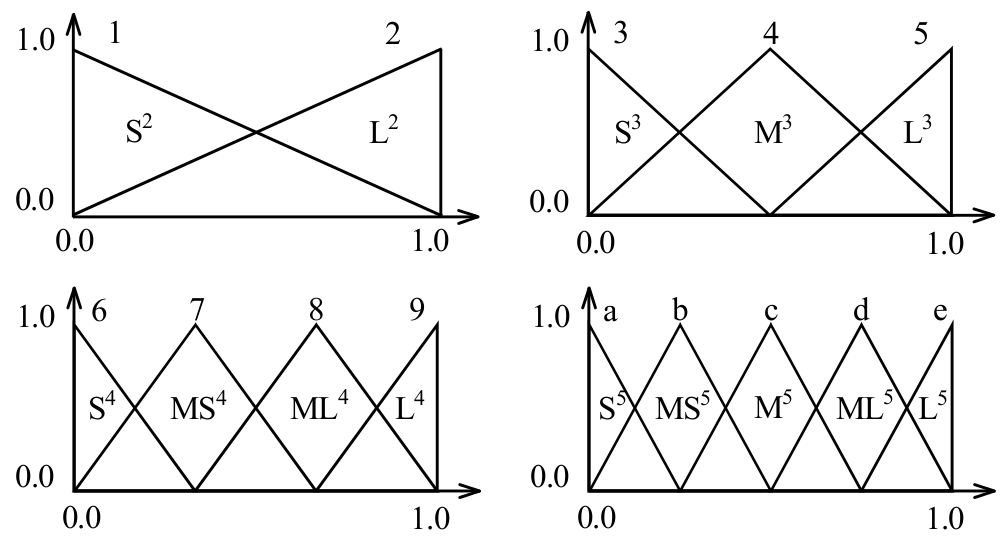
\includegraphics[width=\textwidth]{fig/fuzzy_example.png}
    \end{center}
    \caption{Example fuzzy partition set for an attribute}
    \label{fig:fuzzy_example}
\end{figure}
For classification task single fuzzy rule is of the following form
\cite{bib30}, \cite{bib20}:
$$R_r:\, IF\, x_1=A_{r1}\, AND\, x_2=A_{r2}\, AND\, \ldots\, AND\, x_d=A_{rd}\, THEN\,
class\, C_r\, with \, CF_r$$
where $x=(x_1, x_2, \ldots, x_d)$ is a $d$-dimensional pattern vector; $A_{ri}$
is an antecedent fuzzy set with a linguistic label (taking into account the
example from \ref{fig:fuzzy_example} $A_{ri}$ can have one label from the set
$\{1, 2, \ldots, 9, a, b, \ldots, e \}$); $C_r$ is a consequent fuzzy set
determining the class label $\{1, \ldots, m\}$, $CF_r$ is a rule strength; $r$
denotes the number of the rule from the set of all possible rules $\{1, \ldots, N_{rule}\}$. 

In simulations presented in this paper $N_{rule}$ was set to ten. In this place it should be
explained why this particular number was chosen. In the literature it is recommended to
use $N_{rule}$ rather small because for greater $N_{rule}$ algorithm's search
abilities are deteriorated significantly \cite{bib4}, \cite{bib11}.
Additionally, special tests were performed to determine the optimal number of
rules in author's software. From researches where $N_{rule}$ was changed from 5
to 50 the best results were obtained for $N_{rule}=10$.


\paragraph{Rule generation}
\label{cha:Fuzzy_logic_rule_generation}
The process of rule generation for fuzzy logic without the expert knowledge is
complex and can be done in couple steps. At first, using available
training set, generate randomly $N_{rule}$ rules. For
each training pattern $x_p$ calculate the compatibility grade of a single rule
connected with antecedent part $A_r = (A_{r1}, A_{r2}, \ldots, A_{rd})$ using
the product operator of each membership function $\mu_{A_{ri}}$ determined for
$A_{ri}$:
\begin{equation}
    \mu_{A_r}(x_p)=\mu_{A_r1}(x_p)\cdot\mu_{A_r2}(x_p)\cdot\ldots\mu_{A_rd}(x_p)
    \label{eq:mu_product}
\end{equation}
If we know how to calculate the compatibility grade of each training pattern
now we can determine $C_r$ and $CF_r$ for each rule. The fuzzy probability
$P(class\, j|A_r)$ of class $j$, $j=(1, \ldots, m)$ indicating how pattern $x$ can be associated with class $j$ 
is given by eq. (\ref{eq:fuzzy_probability}) \cite{bib30}:
\begin{equation}
    Pr(class \, j|A_r) = \frac{\sum\limits_{x_p \in class\,
    j}\mu_{A_r}(x_p)}{\sum\limits_{p=1}^m\mu_{A_r}(x_p)}
    \label{eq:fuzzy_probability}
\end{equation}
For the $r$-th rule $R_r$ the label of class is assigned according to the
winning rule, which means that the label with maximal probability is chosen:
\begin{equation}
    R_r: C_r = max\limits_{j=\{1, \ldots, m\}}\{Pr(class\,j|A_r)\}
    \label{eq:fuzzy_max}
\end{equation}
In the learning phase it can happen that rule $R_r$ can be activated by
patterns coming from different classes. To ensure the proper classification, each
rule has a strength factor which tells how precisely rule $R_r$ predicts the
consequent class $j$.
\begin{equation}
    R_r: CF_r=Pr(class\, j|A_r) - \sum\limits_{j=1, j\neq C_r}^MPr(class\,j|A_r)
    \label{eq:fuzzy_strength}
\end{equation}
If $CF_r$ in eq. (\ref{eq:fuzzy_strength}) is negative then rule $R_r$ is
denoted as \textit{dummy} and is not taken for further reasoning, otherwise it is used in
defuzzification process to determine the final class label \cite{bib18}, \cite{bib26}.
\paragraph{Fuzzy reasoning}
\label{cha:Fuzzy_reasoning}
Let assume that $N_{rule}$ fuzzy rules are generated with indicators $C_r$,
$CF_r$ determined by eq. (\ref{eq:fuzzy_max}), (\ref{eq:fuzzy_strength}). 
Then the process of classification is done as follows:
\begin{equation}
    \Psi(S, x_p) =  C_q \leftarrow max_{j=\{1,\ldots,
    M\}}\{\mu_{A_{q}}(x_p)\cdot CF_r\}
    \label{eq:fuzzy_classification}
\end{equation}
The label of the class for unknown pattern is determined by a winner rule $R_w$
that has the maximum compatibility grade and the rule strength $CF_r$.

If multiple fuzzy rules have the same maximum product $\mu_{A_r}$ but different
consequent classes then the classification is rejected. The same action is
taken if no fuzzy rule is compatible with the incoming pattern $x_p$.

\paragraph{Genetic algorithm for  fuzzy algorithm construction}
\label{cha:Fuzzy_logic_genetic_algorithm}
In this section genetic algorithm will be described in greater details. This
algorithm was used to generate an initial number $N_{rule}$ set of fuzzy rules for
classification. 
Basic assumptions:
\begin{itemize}
    \item fuzzy rule encoding is the same as presented in section
        \ref{cha:Fuzzy_logic_basic_problem_formulation},
    \item training data set is given with $N$ patterns,
    \item triangular membership functions are used and are described by 2-tuple
        $(a, b)$, where $a$ is the center value (where $\mu(x)=1$), and
        $b$ determines left and right extend of membership function,
        respectively,
        \begin{equation}
            \mu(x) = 
            \begin{cases}
                \frac{-1}{b}\cdot x + \frac{a+b}{b} &
                x \geq a \, and \, x \leq (a+b) \\
                \frac{1}{b}\cdot x - \frac{a-b}{b} &
                x \geq (a - b)\, and\, x < a \\
                0 & otherwise
            \end{cases}
            \label{eq:fuzzy_function}
        \end{equation}
    \item possible partitions of the feature space are determined in the same
        way as in the example presented in fig. \ref{fig:fuzzy_example},
    \item genetic algorithm uses standard operations such as cross-over,
        mutation, population generation, fitness evaluation,
    \item as the template for genetic fuzzy algorithm Michigan approach is
        used which means that we have $N_{rule}$ number of individuals in the
        population.
\end{itemize}
Next few step will present the whole structure of genetic algorithm used in
fuzzy logic:
\begin{itemize}
    \item chromosome representation and encoding: 
        \begin{itemize}
            \item each individual represents a single fuzzy rule $R_r$ from the
                set of containing $N_{rule}$ rules.
                The length of the chromosome is the same as the number of 
                attributes describing the pattern $x$. Each allele has value
                determining which linguistic variable is used in the current
                rule. Reconsider Iris dataset which is a $4$-dimensional
                classification problem where for each attribute $14$
                membership functions plus one variable telling to omit the
                attribute (called $DON'T \,USE$) are generated. 
                An exemplary individual can be as follows:
                $$1|c|DON'T \;USE|4||1|0.85$$
                Above individual can be decoded into rule presented in fig.
                \ref{fig:fuzzy_rule}
                \begin{figure}[H]
                    \begin{center}
                        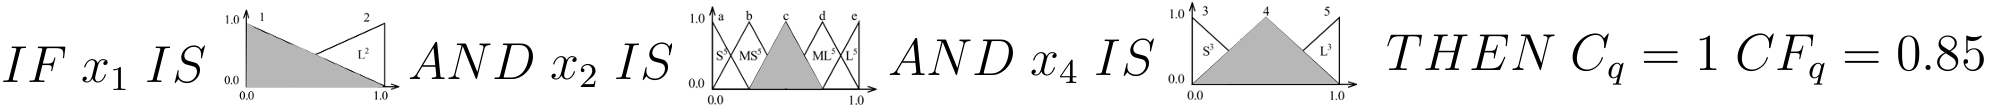
\includegraphics[width=\textwidth]{fig/fuzzy_rule.png}
                    \end{center}
                    \caption{Example rule decoded from the individual
                    chromosome (attribute $x_3$ was omitted in this rule)}
                    \label{fig:fuzzy_rule}
                \end{figure}  
                This rule assigns patterns to class $j=1$ with the strength equal to 0.85.
        \end{itemize}
    \item individual evaluation
        \begin{itemize}
            \item to ensure proper genetic algorithm process an appropriate
                fitness function must be defined \cite{bib10}, \cite{bib21}. 
                Firstly the nature of pattern recognition task must be taken 
                into account and secondly the structure of the fuzzy algorithm. 
                Generally, the main goal is
                to generate rules with the highest $CF_r$ grade, the smallest number
                of attributes and the highest classification rate. Fitness
                function is given by eq. (\ref{eq:fuzzy_fitness})
                \begin{equation}
                    F_{fg} = w_1\cdot NC + w_2\cdot NNC + (\frac{1}{NOF})^2 +
                    w_3\cdot CF
                    \label{eq:fuzzy_fitness}
                \end{equation}
                where $w_1$, $w_2$ are weights for a reward and punishment to
                the rule based on the classification result (in simulations
                $w_1=5$, $w_2=10$); $NC$ and $NNC$ are
                the numbers of correctly recognized and misclassified patterns
                by a particular rule, respectively; $NOF$ is the number of
                attributes used by the rule (in the above example $NOF=3$);
                $CF$ is the strength factor of the rule and $w_3$ is the
                weight (in the simulations $w_3=10$).
                The best individuals are those which maximize function
                $F_{fg}$. It is worth noting that function $F_{fg}$ was
                proposed by author as the extension for most commonly met
                functions in the literature where only the number of correctly
                recognized patterns is taken into account in individuals
                evaluations. In this thesis the complexity of the rule and its
                strength had to be reconsidered additionally.
        \end{itemize}
    \item cross-over
        \begin{itemize}
            \item from the whole population two individuals are chosen
                randomly to constitute parents for further reproduction. With a
                probability of $0.5$ each allele is picked either from mother
                or father chromosome. In this way two new
                individuals are generated (see example in fig.
                \ref{fig:cross_over}),
                \begin{figure}[H]
                    \begin{center}
                        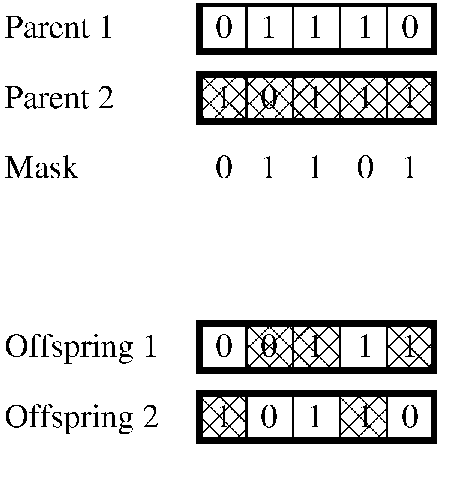
\includegraphics[width=0.6\textwidth, height=0.5\textwidth]{fig/cross_over.png}
                    \end{center}
                    \caption{Cross-over operation used in genetic algorithm}
                    \label{fig:cross_over}
                \end{figure}
        \end{itemize}
    \item mutation
        \begin{itemize}
            \item in the particular generation one chromosome is chosen
                randomly and later in each allele new membership function is
                taken from other possible functions. For example if in the first
                allele the first membership function is chosen the set of
                candidates is given by $\{2, \ldots, 9, a, \ldots, e, DON'T\,
                USE\}$,
        \end{itemize}
    \item selection
        \begin{itemize}
            \item in genetic algorithm one of the most important issue is how
                to generate next population \cite{bib22}. Here, after the end of one
                generation individuals from the population are merged with
                those created through cross-over and mutation operations.
                Later, the average fitness value $F_{avg}$ is calculated for the whole
                set. In the end those individuals are transfered to the next
                generation which fulfill the condition that their fitness indicator $F_{fg}$ 
                is greater than the average $F_{fg} \ge F_{avg}$,
        \end{itemize}
\end{itemize}
Of course it can happen that for cross-over and mutation operator
newly-generated individual will be invalid (the whole chromosome contains only
$DON'T\; USE$ linguistic variables). In such a situation rule is rejected and
the whole generation process is repeated again.

Table \ref{tab:fuzzy_genetic_parameters} presents basic genetic algorithm parameters.
Optimal values were determined during simulations by trial and error method.
\begin{table}[H]
    \caption{Parameter settings for genetic algorithm used in fuzzy logic}
    \centering
    \begin{tabular}{|c|c|}
        \hline
        Parameter & value \\ \hline \hline
        $N_{rule}$ & 10 \\ \hline
        $N_{replace}$ & $N_{rule}/2$ \\ \hline
        Crossover probability & 0.9 \\ \hline
        Mutation probability & 0.3 \\ \hline
        Generations & 500 \\ \hline
    \end{tabular}
    \label{tab:fuzzy_genetic_parameters}
\end{table}

\subsubsection{Rough sets and genetic algorithm}
\label{cha:Multistage_rough_genetic}
Rough sets algorithm presented in section \ref{cha:Algorithm_construction_rough_set} uses an 
arbitrary chosen step of granulation and each attribute has the same
granulation intervals. In some cases this approach gives good results, but in more
complex problems algorithm efficiency is low \cite{bib24}, \cite{bib29}. Additionally, the basic rough set
algorithm uses all attributes for rule construction.

Finding the optimal attribute reduct and rough set partition is $NP$ problem \cite{bib19}, \cite{bib1}.
To overcome this obstacle a genetic algorithm is used in the similar way as in section
\ref{cha:Fuzzy_logic_genetic_algorithm}. Now, a single individual describes the
partition for each attribute independently. Reconsider individual encoding for
$4$-dimensional Iris dataset. The number of granulation intervals for each attribute is
chosen from the set $\{1, 2, \ldots, K_{max}\}$, where $K_{max}$ is the maximum
value of discretization. Additionally, $DON'T\; USE$ variable is used to
determine that a given attribute is excluded from the rule. The example of
individual is given below:
$$|2|DON'T \; USE|K_{max}|3||120$$
It means that the first feature is divided into two intervals, the second is
not used and the third and fourth are discretized into $K_{max}$ and 3
intervals, respectively. The fitness indicator of this individual is $120$.
To evaluate individual the following fitness function given by eq.
(\ref{eq:rough_fitness}) is proposed:

\begin{equation}
    F_{rg} = w_1\cdot NC + w_2\cdot NNC + (\frac{1}{NOF}) +w_3\cdot (\frac{1}{NOCR})^2
    \label{eq:rough_fitness}
\end{equation}
,where $w_1$, $w_2$ are weights for a reward and punishment to
the individual on the classification result ($w1=5$, $w_2=10$); $NC$ and $NNC$ are
the numbers of correctly recognized and misclassified patterns; $NOF$ is the number of
attributes used by the rule (in the example above $NOF=3$);
$NOCR$ is the number of \textit{certain} rules which are derived from
partition given by the particular individual; $w_3$ is the weight (in the simulations
$w_3=10$).

The whole procedure of constructing genetic rough sets algorithm can be summarized in few steps:
\begin{enumerate}
    \item Determine the maximum partition value for each attribute $K_{max}$. In
        this thesis $K_{max}$ is the same for all features and is equal to 7, 
    \item Generate $N_{pop}$ individuals by randomly assigning value from the
        set $\{1, 2, \ldots, K_{max}, \, DON'T\; USE\}$ to each allele in the
        chromosome,
    \item Treat each individual as a rough set partition and calculate lower,
        upper approximations and the boundary region. Evaluate individual using
        fitness function $F_{rg}$,
    \item Generate $N_{replace}$ individuals using genetic operators and merge
        with the current population,
    \item Choose $N_{pop}$ individual for the next generation
    \item If stopping criteria is not fulfilled go to $2$,
\end{enumerate}
Cross-over and mutation operations are done in the same way as presented in
section \ref{cha:Fuzzy_logic_genetic_algorithm}. Parameters for genetic algorithm 
used in this section are presented in table \ref{tab:rough_genetic_parameters}:
\begin{table}[H]
    \caption{Parameter settings for genetic algorithm used in rough sets}
    \centering
    \begin{tabular}{|c|c|}
        \hline
        Parameter & value \\ \hline \hline
        $N_{pop}$ & 10 \\ \hline
        $N_{replace}$ & $N_{pop}/2$ \\ \hline
        Crossover probability & 0.9 \\ \hline
        Mutation probability & 0.2 \\ \hline
        Generations & 100 \\ \hline
    \end{tabular}
    \label{tab:rough_genetic_parameters}
\end{table}
In case of genetic algorithm for rough set $100$ generations were sufficient to
obtain reliable results.
\subsubsection{Hybrid rough sets and fuzzy logic algorithm}
\label{cha:Multistage_rough_fuzzy}
Multistage classifier created in this thesis can be divided into three phases:
\begin{enumerate}
    \item rough sets classifier construction using genetic algorithm presented
        in section \ref{cha:Multistage_rough_genetic},
    \item fuzzy logic classifier construction with rule generation by heuristic
        approach described in \ref{cha:Fuzzy_logic_genetic_algorithm},
    \item pattern recognition using sequential hybrid classifier,
\end{enumerate}
Each step plays an important role in the whole process and affects the final
classification accuracy \cite{bib12}, \cite{bib27}, \cite{bib32}. Proper parameters of genetic algorithm are especially
important. The whole hybrid algorithm can be summarized in the following steps:
\begin{enumerate}
    \item Divide available dataset into three separated subsets: the first for
        genetic algorithm operation, the second and third as training and
        testing.
    \item Train rough sets, fuzzy logic classifiers
    \item Classify pattern using rough sets algorithm:
        \begin{itemize}
            \item If pattern is classified by a \textit{certain} or
                \textit{possible} rule then it is a final label
            \item If no proper rule is found or more than one rule have the same
                strength but different label then pattern is rejected and
                processed by fuzzy logic classifier.
        \end{itemize}
\end{enumerate}
An illustrative scheme of hybrid classifier is presented in fig. \ref{fig:schematic}.
\begin{figure}[H]
    \begin{center}
        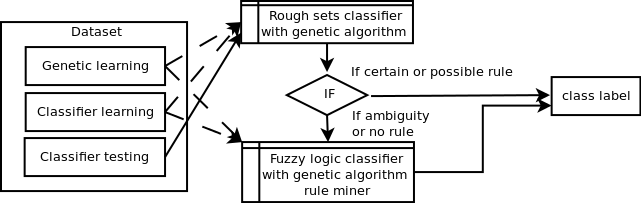
\includegraphics[width=\textwidth]{fig/diagram.png}
    \end{center}
    \caption{Diagram presenting how hybrid classifier works}
    \label{fig:schematic}
\end{figure}
\subsubsection{Difference between rough sets and fuzzy logic reasoning}
\label{cha:Difference}
At the end of this section the difference between rough sets and fuzzy logic should 
be explained more deeply. In rough sets algorithm we provide discretization for the 
whole feature and the number of generated decision rules is equal the number of objects 
in the set. In previous section it was stated that rough sets can be associated with table. 
Opposite to rough sets algorithm is fuzzy logic in which the number of rules is much smaller 
and in this thesis it is 10. We do not want to partition the whole feature space into fuzzy 
sets, instead we pick only those membership functions which ensure the greatest compatibility 
grade with training patterns.
